\documentclass[a4paper, 11pt]{article}
\usepackage{amsmath}
\usepackage{graphicx}
\usepackage{geometry}
\usepackage{listings}
\geometry{scale=0.8}

\title{	
\normalfont \normalsize
\textsc{School of Data and Computer Science, Sun Yat-sen University} \\ [25pt] %textsc small capital letters
\rule{\textwidth}{0.5pt} \\[0.4cm] % Thin top horizontal rule
\huge  The Water Jug Riddle\\ % The assignment title
\rule{\textwidth}{2pt} \\[0.5cm] % Thick bottom horizontal rule
\author{Shixuan Lee 15336085}
\date{\normalsize\today}
}


\begin{document}
\maketitle
\newpage
\tableofcontents
\newpage
\section{Problem Description}
This is a problem that is prominently featured in the film Die Hard With a Vengeance. You have a 3-gallon and a 5-gallon jug that you can fill from a fountain of water. The problem is to fill one of the jugs with exactly 4 gallons of water. How do you do it?

This is the solution (not the only solution):
\begin{enumerate}\setlength{\itemsep}{-\itemsep}
\item Fill up the 3-gallon jug
\item Transfer to the 5-gallon jug
\item Fill up the 3-gallon jug again
\item Transfer water to fill up the 5-gallon jug, leaving 1 gallon in the 3-gallon jug
\item Empty out the 5-gallon jug
\item Transfer the 1 gallon to the 5-gallon jug
\item Fill up the 3-gallon jug and transfer that to the 5-gallon jug
\item The 5-gallon jug contains 4 gallons of water
\end{enumerate}
The sequence here is:

$(0, 3)->(3, 0)->(3, 3)->(5, 1)->(0, 1)->(1, 0)->(1, 3)->(4,0)$

\section{Task}
\begin{enumerate}
\item Please solve the Water Jug Riddle by using A* search algorithm.
\item The reference code can be found in \textsf{ReferenceWaterJub.rar}, which you can use to accomplish this task by adding your A* heuristic function.
\item Don't forget to run at least 3 instances to verify the correctness of your programs.
\item Write the related codes and take a screenshot of the running results in the file named \textsf{E03\_YourNumber.pdf}, and send it to \textsf{ai\_2017@formail.com}
\end{enumerate}
\section{codes}
\lstset{language=C++}
\lstset{breaklines=true}
\begin{lstlisting}
#include <bits/stdc++.h>
#include <cmath>
#include <queue>
using namespace std;
class nodes{
	public: 
		pair<int,int> p;
		int fval;
		int depth;
		string s;
		bool operator<(const nodes &s) const{
			return fval > s.fval;
		}
		bool operator>(const nodes &s)const{
			return fval < s.fval;
		}
		bool operator==(const nodes &s)const{
			return fval == s.fval;
		}
};

string makestring(int a,int b){
	std::stringstream out1;
	std::stringstream out2;
	string t1,t2,str;
    out1 << a;
    t1 = out1.str();
    out2 << b;
    t2 = out2.str();
    str = "("+t1+","+t2+")";
    return str;
}

int gcd(int x, int y){
	return y == 0? x: gcd(y, x % y);
}

bool soluble(int fir, int sec, int tar){
	return tar == 0 || (fir + sec > tar && tar % gcd(fir, sec) == 0);
}

int getf(nodes temp, int s, int e){
	int g = abs(temp.p.first - s) + abs(temp.p.second - e);
	int h = temp.depth;
	return g + h;
}

int main()
{
	//int counter = 0;
    ios::sync_with_stdio(false);
    //pair<int,int> cap,ini,final;
    nodes cap,ini,final;
    ini.p.first=0,ini.p.second=0,ini.fval=0,ini.depth=0;
    ini.s = makestring(ini.p.first,ini.p.second);
    //Input initial values
    cout<<"Enter the capacity of 2 jugs\n";
    cin>>cap.p.first>>cap.p.second;
    //input final values
    cout<<"Enter the required jug config\n";
    cin>> final.p.first >>final.p.second;
    bool sol;
    sol = soluble(cap.p.first, cap.p.second, final.p.first);
    if(sol == 0){
    	cout << "No Solution.\n" ;
    	return 0;
    }
    //Using A* to find the answer
    priority_queue<nodes> open;
    queue<nodes> close;
    open.push(ini);
    nodes jug;
    while(!open.empty()){
    	jug = open.top();
    	open.pop();
    	close.push(jug);
    	if(jug.p.first == final.p.first && jug.p.second == final.p.second){
    		cout<<jug.s<<endl;
	  		break;
    	}
    	nodes temp = jug;
    	//Fill 1st Jug
    	if(jug.p.first<cap.p.first){
			temp.p = make_pair(cap.p.first,jug.p.second);
			temp.s = jug.s + makestring(temp.p.first,temp.p.second);
			temp.depth = jug.depth + 1;
			temp.fval = getf(temp, final.p.first, final.p.second);
			open.push(temp);
    	}
    	//Fill 2nd Jug
    	if(jug.p.second<cap.p.second){
			temp.p = make_pair(jug.p.first,cap.p.second);
			temp.s = jug.s + makestring(temp.p.first,temp.p.second);
			temp.depth = jug.depth + 1;
			temp.fval = getf(temp, final.p.first, final.p.second);
			open.push(temp);
    	}
    	//Empty 1st Jug
    	if(jug.p.first>0){
			temp.p = make_pair(0,jug.p.second);
			temp.s = jug.s + makestring(temp.p.first,temp.p.second);
			temp.depth = jug.depth + 1;
			temp.fval = getf(temp, final.p.first, final.p.second);
			open.push(temp);
    	}
    	//Empty 2nd Jug
    	if(jug.p.second>0){
			temp.p = make_pair(jug.p.first,0);
			temp.s = jug.s + makestring(temp.p.first,temp.p.second);
			temp.depth = jug.depth + 1;
			temp.fval = getf(temp, final.p.first, final.p.second);
			open.push(temp);
    	}
    	//Pour from 1st jug to 2nd until its full
    	if(jug.p.first>0 && (jug.p.first+jug.p.second)>=cap.p.second){
    		temp.p = make_pair((jug.p.first-(cap.p.second-jug.p.second)),cap.p.second);
    		temp.s = jug.s + makestring(temp.p.first,temp.p.second);
    		temp.depth = jug.depth + 1;
			temp.fval = getf(temp, final.p.first, final.p.second);
			open.push(temp);
    	}
    	//Pour from 2nd jug to 1st until its full
    	if(jug.p.second>0 && (jug.p.first+jug.p.second)>=cap.p.first){
    		temp.p = make_pair(cap.p.first,(jug.p.second-(cap.p.first-jug.p.first)));
    		temp.s = jug.s + makestring(temp.p.first,temp.p.second);
    		temp.depth = jug.depth + 1;
			temp.fval = getf(temp, final.p.first, final.p.second);
			open.push(temp);
    	}
    	//Pour all water from 1st to 2nd
    	if(jug.p.first>0 && (jug.p.first+jug.p.second)<=cap.p.second){
    		temp.p = make_pair(0,jug.p.first+jug.p.second);
    		temp.s = jug.s + makestring(temp.p.first,temp.p.second);
    		temp.depth = jug.depth + 1;
			temp.fval = getf(temp, final.p.first, final.p.second);
			open.push(temp);
    	}
    	//Pour from 2nd jug to 1st until its full
    	if(jug.p.second>0 && (jug.p.first+jug.p.second)<=cap.p.first){
    		temp.p = make_pair(jug.p.first+jug.p.second,0);
    		temp.s = jug.s + makestring(temp.p.first,temp.p.second);
    		temp.depth = jug.depth + 1;
			temp.fval = getf(temp, final.p.first, final.p.second);
			open.push(temp);
    	}
    }
	return 0;
}

\end{lstlisting}
\section{Results}
\centering
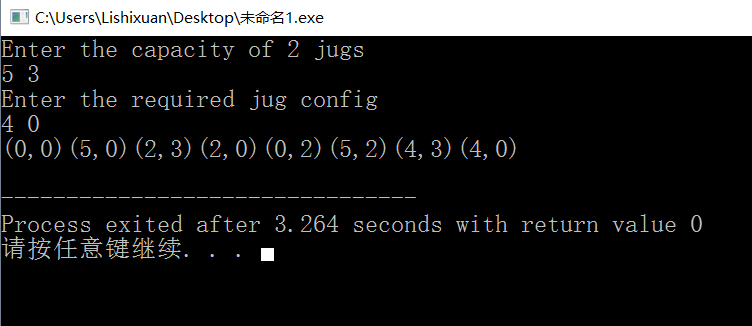
\includegraphics[width=15cm]{waterjug1.png}
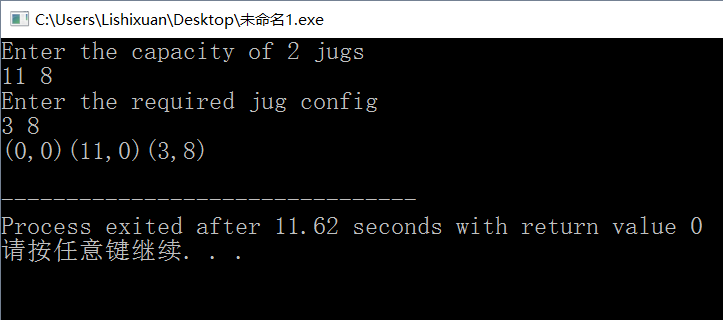
\includegraphics[width=15cm]{waterjug2.png}
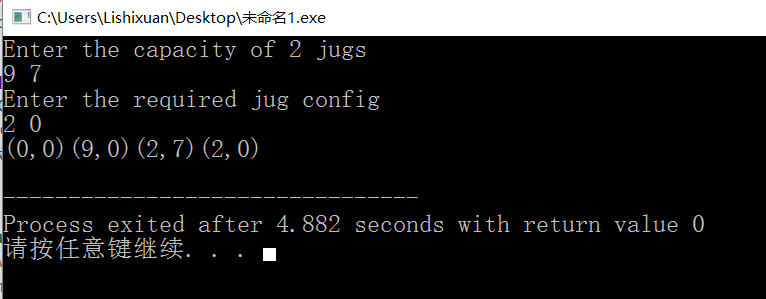
\includegraphics[width=15cm]{waterjug3.png}
%\tableofcontents
%\newpage

\end{document} 